\documentclass{beamer}
\usetheme[pageofpages=of,% String used between the current page and the
                         % total page count.
          bullet=circle,% Use circles instead of squares for bullets.
          titleline=true,% Show a line below the frame title.
          alternativetitlepage=true,% Use the fancy title page.
	  titlepagelogo=logo-circl.pdf,% Logo for the first page.
%          watermark=watermark-polito,% Watermark used in every page.
%          watermarkheight=100px,% Height of the watermark.
%          watermarkheightmult=4,% The watermark image is 4 times bigger
                                % than watermarkheight.
          ]{Torino}

\usepackage[utf8]{inputenc}
\usepackage{listings}
\usepackage{graphicx}
\usepackage{siunitx}
\usepackage{booktabs}
\usepackage[font=small,labelfont=bf]{caption}
\usepackage{transparent}
\usepackage{verbatim}
\usepackage{tabularx}
\lstset{ 
  backgroundcolor=\color{white},   % choose the background color; you must add \usepackage{color} or \usepackage{xcolor}
  basicstyle=\footnotesize,        % the size of the fonts that are used for the code
  breakatwhitespace=false
}

\usepackage{tikz}
\usetikzlibrary{shapes,arrows}

\author{TEAM CIRCL\\ \emph{TLP:CLEAR}}
\title{NGSOTI (Next Generation Security Operator Training Infrastructure)}

\subtitle{Introduction to Incident Response}
\institute{info@circl.lu}
\date{2025-01-28}

\begin{document}
% DO NOT COMPILE THIS FILE DIRECTLY!
% This is included by the other .tex files.

\begin{frame}
    \maketitle
\end{frame}

\begin{frame}
\frametitle{Outline}
\tableofcontents
\end{frame}
\section{Welcome}


\begin{frame}
	\frametitle{Welcome and Introduction}
	\framesubtitle{Interactions during the training}
	\begin{itemize}
		\item Collaboration during the training.
		\item Interrupt the training at any point in time if you have important questions.
		\item Write your questions in the hdoc.
		\item Use the collaborative notes to share information.
		\item collaborative notes that can be downloaded and converted in docx or PDF.
	\end{itemize}
\end{frame}

\begin{frame}
	\frametitle{Welcome}
	\framesubtitle{Interactions with the audience}
	\begin{itemize}
		\item Round table.
		\item Purpose make this training useful.
		\item What are your area of expertise?
		\item What do you expect from this course?
	\end{itemize}
\end{frame}


\section{CIRCL background and services}
\begin{frame}
 	\frametitle{CIRCL background and services}
 
\includegraphics[scale=0.5]{logo-circl.pdf}
 \begin{itemize}
     \item The Computer Incident Response Center Luxembourg (CIRCL\footnote{\url{https://www.circl.lu/}}) is a government-driven initiative designed to provide a systematic response facility to computer security threats and incidents.
 \item CIRCL is the CERT for the {\bf private sector}, communes and non-governmental entities in Luxembourg.
 \item Started operation under Economic Interest Group in September 2010.
 \item Under NIS regulation (duties defined in the law of 28 may 2019 defined in Mémorial A $N^{o}$ 372 of the 31 May 2019).
 \end{itemize}
\end{frame}

\begin{frame}
\frametitle{CIRCL background and services}
\framesubtitle{CIRCL Missions 1/2}
\begin{itemize}
\item Provide a {\bf systematic and pragmatic response} facility to cyber security incidents.
\item {\bf Support economical sector} to recover quickly and efficiently from cyber security incidents.
\item Minimize cyber security incident-based losses, theft of information and disruption of services.
\end{itemize}
\end{frame}

\begin{frame}
\frametitle{CIRCL background and services}
\framesubtitle{CIRCL Missions 2/2}
\begin{itemize}
\item {\bf Gather information/intelligence related to incident handling} to better prepare future incidents management and provide optimized protection for systems and data.
\item Coordinate communication among national and international incident response teams\footnote{FIRST.org, CSIRTs network, TF-CSIRT...} during security emergencies and to help prevent future incidents.
\item Provide a security related {\bf information sharing community} and warning system for national ICT users and international partners.
\item Foster knowledge and awareness exchange\footnote{\url{https://www.circl.lu/pub/}} in cyber security.
\end{itemize}
\end{frame}


\begin{frame}
\frametitle{CIRCL background and services}
\framesubtitle{CIRCL Services - Incident Coordination}
    \begin{itemize}
        \item Incident handling\footnote{\url{https://www.circl.lu/opendata/statistics/}} for reported ICT incidents via different medium (e.g. International CSIRT channel, national incident report,...).
        \item Incident identification and triage.
        \item Technical investigation including information correlation (e.g. Security vulnerability/incidents matching, similar incident resolution,...).
        \item Incident coordination might also include vulnerability handling and {\bf coordinated vulnerability disclosure\footnote{\url{https://www.circl.lu/pub/responsible-vulnerability-disclosure/}}} (e.g. software vulnerability related to an incident).
    \end{itemize}
\end{frame}

\begin{frame}
\frametitle{CIRCL background and services}
\framesubtitle{CIRCL and Open Source Tooling}
    \begin{itemize}
        \item From the early beginning of CIRCL, {\bf developing tools and software} for our use-cases should be available to others\footnote{{\it Public Money, Public Code}}.
        \item For all software developed, associated {\bf services}\footnote{publicly accessible or restricted access services} are available.
        \item {\bf Producing intelligence} from the services available.
        \item In 2024, CIRCL maintain more than 14 open source projects\footnote{\url{https://opensource-metrics.circl.lu/}} (250+ official git repositories).
    \end{itemize}
\end{frame}

\begin{frame}
	\frametitle{CIRCL background and services}
	\framesubtitle{MISP Project and CIRCL}
    \begin{itemize}
        \item CIRCL {\bf leads the development} of the Open Source MISP threat intelligence platform\footnote{\url{https://www.misp-project.org/}} which is used by many military or intelligence communities, private companies, financial sector, National CERTs and LEAs globally.  
        \item {\bf CIRCL runs multiple large MISP communities performing active daily threat-intelligence sharing}.
        \item Private sector such as the financial sector can request access to one or more information sharing communities operated by CIRCL.
    \end{itemize}
\end{frame}

\begin{frame}
	\frametitle{CIRCL background and services}
	\framesubtitle{MISP communities management and hosting}
    	\begin{itemize}
      	 	\item CIRCL provides {\bf different level of MISP hosting} for communities such as CSIRTs, financial sector, mobile operator sector, banking regulator which can include:
           	\begin{itemize}
            		\item Dedicated virtual or physical MISP instance hosted in Luxembourg; 
            		\item MISP software stack maintenance;
            		\item Managing organisation and communities;
            		\item Bootstrapping information and intelligence from feeds or other communities; 
            	\end{itemize}
    	\end{itemize}
\end{frame}

\begin{frame}
	\frametitle{CIRCL background and services}
	\framesubtitle{What is MISP?}
    \begin{center}
        
\includegraphics[width=0.2\linewidth]{pictures/misp-logo.png}
    \end{center}
    \begin{itemize}
        \item MISP is a {\bf threat information sharing} platform that is free \& open source software.
        \item A tool that {\bf collects} information from partners, your analysts, your tools, feeds.
        \item Normalises, {\bf correlates}, {\bf enriches} the data.
        \item Describe and structure complex TTPs\footnote{Tactics, techniques, and procedures.}, course of action or custom intelligence. 
        \item Allows teams and communities to {\bf collaborate}.
        \item {\bf Feeds} automated protective tools and analyst tools with the output.
    \end{itemize}
\end{frame}

\begin{frame}
    \frametitle{CIRCL background and services}
    \framesubtitle{MISP Project - ecosystem overview}

    \begin{itemize}
        \item An open standard\footnote{\url{https://www.misp-standard.org/}}, training materials.
        \item Classification libraries\footnote{\url{https://www.misp-project.org/taxonomies.html}} \& encyclopedia\footnote{\url{https://www.misp-project.org/galaxy.html}} (from threat-actor databases to MITRE ATT\&CK).
        \item \textbf{MISP-specific tools}: Python Wrapper, Enrichment service, misp-guard for air-gapped system, etc.
        \item \textbf{Integration and workflows}: OpenAPI, Workflow blueprints, misp-modules (300+ enrichments), etc.
        \item Open data \& OSINT Feeds.
    \end{itemize}
\end{frame}

\begin{frame}
	\frametitle{CIRCL background and services}
	\framesubtitle{MISP Training materials}
Plethora of content for \textbf{different objectives} and \textbf{use-cases}
    \begin{itemize}
        \item \textbf{MISP Book\footnote{\url{https://www.circl.lu/doc/misp/}}} User guide for day-to-day usage.
        \item \texttt{MISP/misp-training}\footnote{\url{https://github.com/MISP/misp-training}} Main repository for any documentation, training materials or conference talks.
        \item \texttt{MISP/misp-training-lea} Complete e-learning course for Law enforcement.
        \item \textbf{Training video} Topical, feature-focused or 4h e-learning session.
        \item \textbf{Others} Cheatsheets, Best practices, guidelines, compliance\footnote{\url{https://misp-project.org/compliance/}}, etc... 
    \end{itemize}
\end{frame}

\begin{frame}
	\frametitle{CIRCL background and services}
	\framesubtitle{Cerebrate}
    \begin{center}
        
\includegraphics[width=0.20\linewidth]{pictures/cerebrate-logo.png}
    \end{center}
    \begin{itemize}
        \item Cerebrate\footnote{\url{https://www.cerebrate-project.org/}} \footnote{\url{https://cerebrate.misp-project.org}} is an open source platform meant to act as a trusted \textbf{contact information provider}.
        \item Main objectives are \textbf{community management} and \textbf{local tool orchestration}.
        \item \textbf{IAM centric design} including users provisioning.
        \item Local tool \textbf{management} and \textbf{inter-connection} (e.g. MISP).
    \end{itemize}
\end{frame}

\begin{frame}
    \frametitle{CIRCL background and services}
    \framesubtitle{Pandora}
    \begin{center}
        
\includegraphics[width=0.5\linewidth]{pictures/pandora-logo.png}
    \end{center}
    \begin{itemize}
        \item Pandora\footnote{\url{https://github.com/pandora-analysis}} \footnote{\url{https://pandora.circl.lu/}} is an analysis framework to discover {\bf whether a file is suspicious and to conveniently show the results}.
        \item This tool was created out of a partnership with the CERT of a bank in need of a local tool in order {\bf to avoid leaking sensitive information} toward third-parties.
        \item CIRCL develops the open source project, along with operating a public instance for the community and supporting organisations wanting to operate local instances. 
    \end{itemize}
\end{frame}

\begin{frame}
    \frametitle{CIRCL background and services}
    \framesubtitle{Lookyloo}
\begin{itemize}
    \item Lookyloo\footnote{\url{https://github.com/Lookyloo}} \footnote{\url{https://lookyloo.circl.lu/}} is {\bf a safe environment to check, review and analyse urls}.
    \item This forensic tool can be used to analyse potential phishing website but also legitimate sites for understanding the interactions.
\end{itemize}
    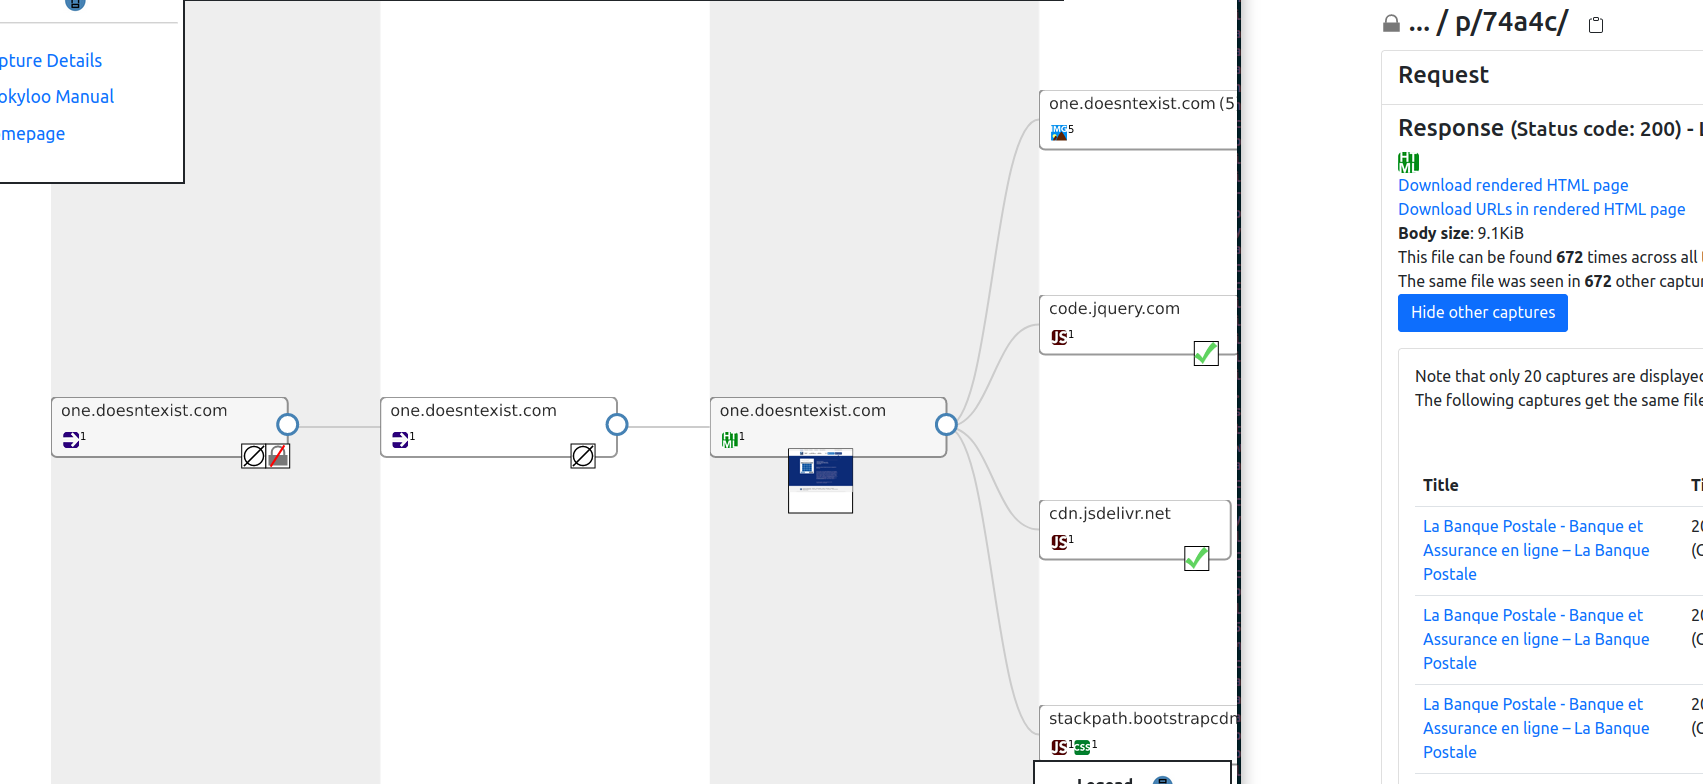
\includegraphics[scale=0.18]{lapostale.png}
\end{frame}

\begin{frame}
    \frametitle{CIRCL background and services}
    \framesubtitle{D4 Project}
    \begin{itemize}
        \item D4 Project\footnote{\url{https://www.d4-project.org/}} is a {\bf large-scale distributed sensor} network to monitor DDoS and other malicious activities relying on an open and collaborative project.
    \end{itemize}
    \begin{center}
    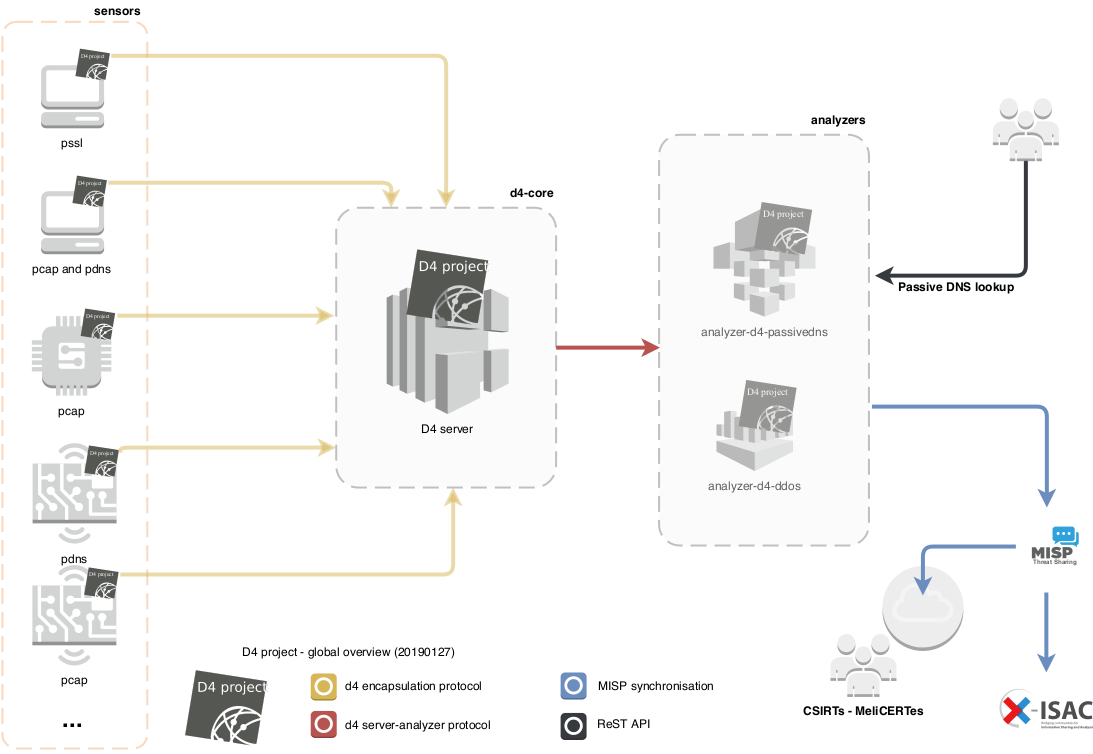
\includegraphics[scale=0.20]{d4-overview.png}
    \end{center}
\end{frame}

\begin{frame}
    \frametitle{CIRCL background and services}
    \framesubtitle{AIL Project}
    \begin{itemize}
        \item AIL Project\footnote{\url{https://ail-project.org/}} is an open source framework to collect, crawl, dig and analyse unstructured data. The framework can be used to find {\bf information leaks}, intelligence, insights and much more. The open source framework includes crawling services (for Tor, I2P) or feeders for specific sources (Telegram, fediverse). 
    \end{itemize}
    \begin{center}
    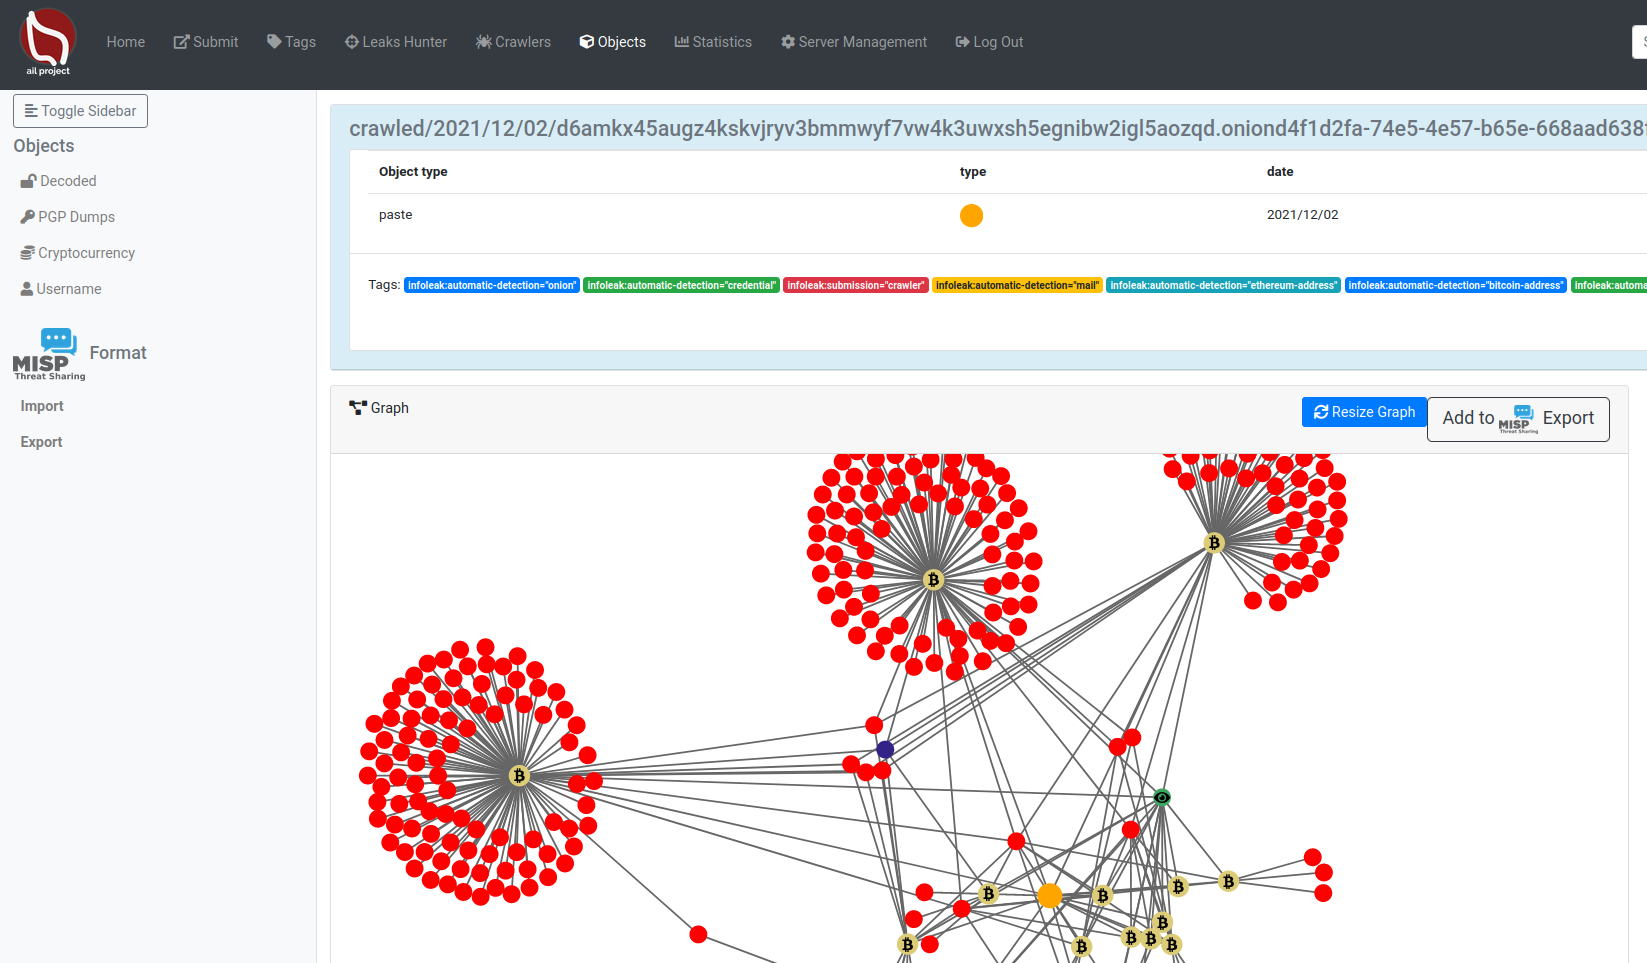
\includegraphics[scale=0.15]{ail-new.png}
    \end{center}
\end{frame}

\begin{frame}
    \frametitle{CIRCL background and services}
    \framesubtitle{Typo Squatting}
    \begin{center}
        
\includegraphics[width=0.17\linewidth]{pictures/typosquatting-logo.png}
    \end{center}
    \begin{itemize}
        \item Typo Squatting\footnote{\url{https://typosquatting-finder.circl.lu/}} is a service to generate, find and assess existing \textbf{fake domain used by adversaries}.
        \item Can be used as a \textbf{standalone Python library}\footnote{\url{https://github.com/ail-project/ail-typo-squatting}} for integration with other tools.
        \item \textbf{Publicly accessible} service to run queries and download the results.
        \item Support many (20+) domain generation algorithms, automatic MISP integration and false-positive detections.
    \end{itemize}
\end{frame}

\begin{frame}
    \frametitle{CIRCL background and services}
    \framesubtitle{Hashlookup}
    \begin{itemize}
        \item Hashlookup\footnote{\url{https://hashlookup.io}} \footnote{\url{https://hashlookup.circl.lu/}} is a public API to lookup hash values against \textbf{known databases of file hashes}.
            \begin{itemize}
                \item include NSRL dataset along with more than 100 sources such as CDNjs, major Linux distributions, snap repositories... 
            \end{itemize}
        \item The service is publicly accessible service or can be used as Bloomfilter datasets to off-line lookups.
        \item Typical usage: During digital forensic investigation to give context and information about the files extracted. 
    \end{itemize}
\end{frame}

\begin{frame}
\frametitle{CIRCL background and services}
\framesubtitle{PassiveDNS, PassiveSSL, PassiveSSH}
    Services providing valuable information during investigation and scenario re-construction.
    \begin{itemize}
        \item \textbf{PassiveDNS}: Historical DNS records database.
        \item \textbf{PassiveSSL}: Historical database of X.509 certificates (query per IP address, certificates).
        \item \textbf{PassiveSSH}: Historical database of SSH keys \& fingerprint (query per IP, fingerprints, banners). 
    \end{itemize}
    \begin{center}
        
\includegraphics[width=0.4\linewidth]{pictures/pssl-logo.png}
        
\includegraphics[width=0.2\linewidth]{pictures/pssh-logo.png}
    \end{center}
\end{frame}



\begin{frame}
 \frametitle{CIRCL background and services}
  \framesubtitle{Vulnerability lookup}
    \begin{figure}[H]
        \centering
        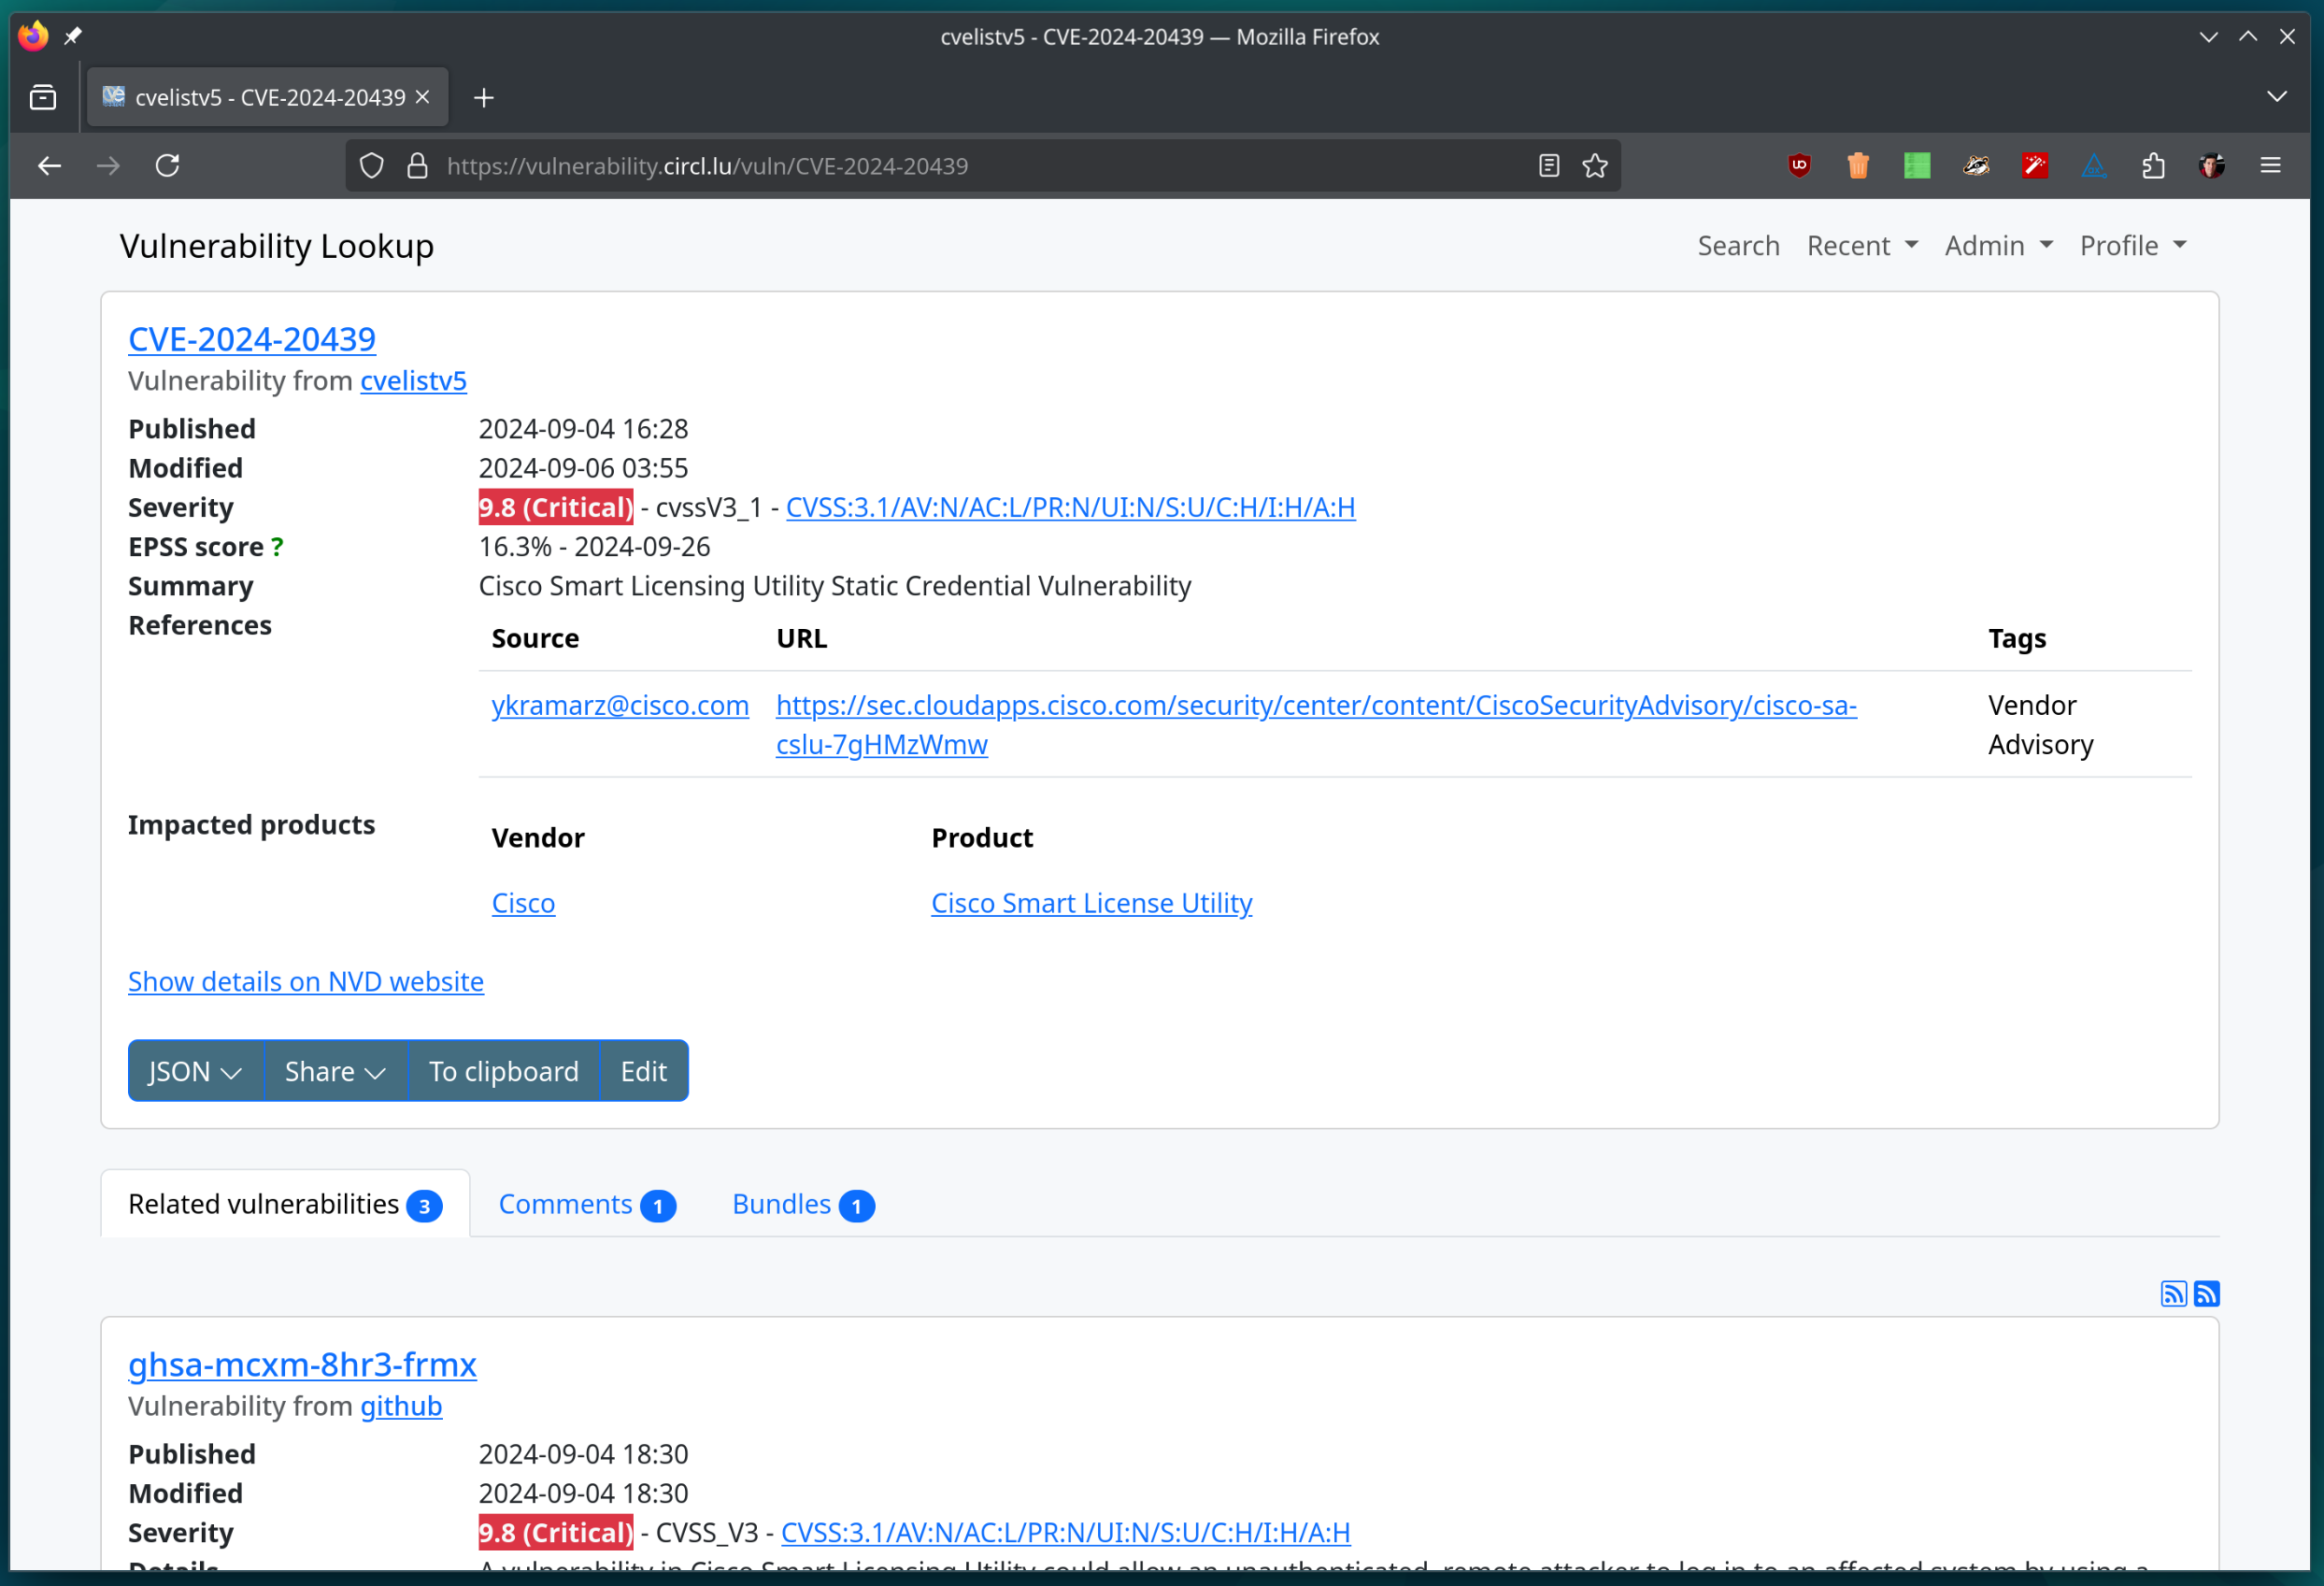
\includegraphics[width=0.77\textwidth]{vulnerability.png}
        \caption{A vulnerability with its details, correlations, comments, and bundles.}
        \label{fig:vulnerability}
    \end{figure}
\end{frame}


\begin{frame}
 \frametitle{CIRCL background and services}
  \framesubtitle{Onion lookup}
    \begin{figure}[H]
        \centering
        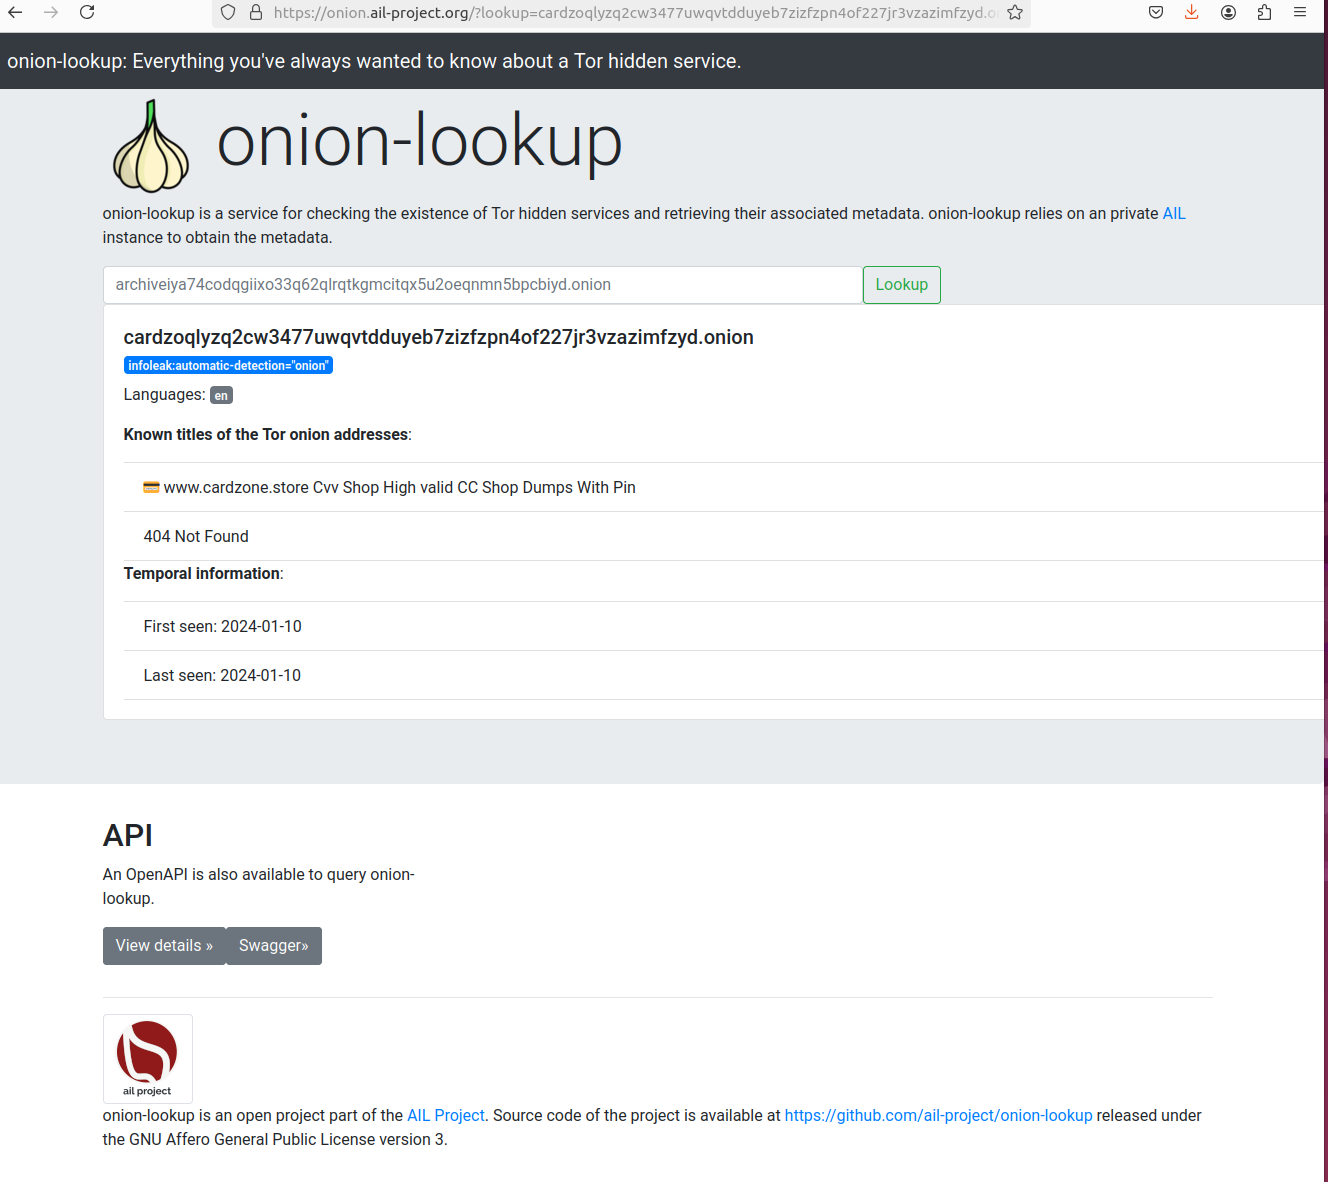
\includegraphics[width=0.77\textwidth]{onion.png}
        \caption{ onion-lookup service}
	\label{onion}
    \end{figure}
       onion-lookup is a service for checking the existence of Tor hidden services and retrieving their associated metadata. onion-lookup relies on an private AIL instance to obtain the metadata.
\end{frame}


\section{Introduction}

\begin{frame}
	\frametitle{Introduction}
	\framesubtitle{Dependencies of incident response training}
	\begin{itemize}
		\item On the capabilities of the team
		\begin{itemize}
			\item In house incident response.
			\item Rely on external entities.
			\item \alert{Critical: Evaluation of the received data / reports}.
		\end{itemize}
		\item On the infrastructure
		\begin{itemize}
			\item On premises with local IT.
			\item On IT integrator.
			\item Using cloud  infrastructure.
			\item Using software as a service (SaaS).
		\end{itemize}
		\item Bring your Own device policy.
		\item ...
	\end{itemize}
\end{frame}

\begin{frame}
	\frametitle{Introduction}
	\framesubtitle{High level view}
	\begin{itemize}
		\item Definition and importance of incident response.
		\item Common types of cybersecurity incidents (e.g., malware, phishing, ransomware, data leaks, president fraud).
		\item Overview of incident response lifecycle (Preparation, Detection, Containment, Eradication, Recovery, Lessons Learned).
		\item Creation and testing of incident response playbooks
	\end{itemize}
\end{frame}


\begin{frame}
	\frametitle{Introduction}
	\framesubtitle{High level view}
	\begin{block}{Incident Response Team (IRT) Roles and Responsibilities}
		\begin{itemize}
			\item Incident Response Team (IRT) Roles and Responsibilities $\to$ clearly defined borders.
			\item Roles in an IRT: Incident Manager, Security Analysts, Forensic Experts, Legal, and PR team.
    			\item Importance of cross-functional collaboration.
    			\item Defining the chain of command and communication channels.
		\end{itemize}
	\end{block}
\end{frame}

\begin{frame}
	\frametitle{Introduction}
	\framesubtitle{Preparation Phase}
	\begin{itemize}
    		\item Developing and maintaining an Incident Response Plan (IRP).
 		\item Setting up tools for monitoring and detection (SIEM, IDS/IPS, firewalls).
   		\item Importance of regular updates to documentation and procedures.
    		\item Training exercises (e.g., tabletop exercises, simulations).
   		\item Data backup and recovery procedures.
   	\end{itemize}
\end{frame}

\begin{frame}
	\frametitle{Introduction}
	\framesubtitle{Detection and Analysis}
	\begin{itemize}
		\item Identifying signs of potential incidents (e.g., unusual activity, system alerts).
   		\item Log analysis and alert correlation techniques.
   		\item Use of automated detection tools.
  		\item Initial triage and prioritization of incidents based on severity.
	\end{itemize}
\end{frame}

\begin{frame}
	\frametitle{Introduction}
	\framesubtitle{Containment Strategies}
	\begin{itemize} 
    		\item Short-term containment: isolating affected systems to prevent further spread.
    		\item Long-term containment: patching vulnerabilities, monitoring for persistence.
    		\item Importance of minimizing business disruption while containing threats.
	\end{itemize}
\end{frame}

\begin{frame}
	\frametitle{Introduction}
	\framesubtitle{Eradication and Recovery}
	\begin{itemize}
    	 	\item Removing the root cause of the incident (malware, compromised accounts).
    		\item Verifying system integrity and security.
     		\item Safe restoration of systems and services.
    		\item Ensuring the incident does not recur.
	\end{itemize}
\end{frame}

\begin{frame}
	\frametitle{Introduction}
	\framesubtitle{Post-Incident Activities}
	\begin{itemize}
    		\item Conducting a thorough post-incident analysis (forensic investigation, root cause analysis).
    		\item Documenting lessons learned and updating the Incident Response Plan.
    		\item Reporting to stakeholders, including executives and regulatory bodies.
    		\item Reviewing and refining security measures.
	\end{itemize}
\end{frame}

\begin{frame}
	\frametitle{Introduction}
	\framesubtitle{Communication and Reporting}
	\begin{itemize}
    		\item Developing internal and external communication strategies.
    		\item Prepare crisis communication.
    		\item Setup out of band communication channels. The other ones could be intercepted or disrupted.
    		\item Clear communication channels between IT, management, and external partners.
    		\item Regulatory compliance: Reporting incidents to authorities as required (GDPR, NIS,NIS2, DORA etc.).
            \item Inspect the regulator reports in advance and make sure that you can get all the data.
	\end{itemize}
\end{frame}

\begin{frame}
	\frametitle{Introduction}
	\framesubtitle{Continuous Improvement}
	\begin{itemize}
    		\item Regular review and updates to the IRP based on lessons learned.
    		\item Ongoing training for team members to stay updated on evolving threats.
   		\item Scheduling regular mock drills and simulations based on real data.
   	\end{itemize}
\end{frame}

\begin{frame}
	\frametitle{Introduction}
	\framesubtitle{An overview to incident response}
\tikzstyle{block} = [rectangle, draw, fill=blue!20, text width=10em, text centered, rounded corners, minimum height=2em]
\tikzstyle{line} = [draw, -latex']

\centerline{
        \begin{tikzpicture}[scale=1, node distance = 1cm, auto]
        \node [block] (detection) {Detection};
        \node [block,below of=detection] (analysis) {Analysis};
        \node [block,below of=analysis] (containment) {Containment};
        \node [block,below of=containment] (investigation) {Investigation};
        \node [block,below of=investigation] (eradication) {Eradication};
        \node [block,below of=eradication] (postmortem) {Postmortem};
        \path [line] (detection) -- (analysis);
        \path [line] (analysis) -- (containment);
        \path [line] (containment) -- (investigation);
        \path [line] (investigation) -- (eradication);
        \path [line] (eradication) -- (postmortem);
        \end{tikzpicture}
}

\end{frame}

\section{Practical aspects}
\begin{frame}[fragile]
\frametitle{Practical aspects}
\framesubtitle{Nowadays, how is the attacker compromising a PC?}
\tikzstyle{block} = [rectangle, draw, fill=blue!20, text width=10em, text centered, rounded corners, minimum height=4em]
\tikzstyle{line} = [draw, -latex']

\centerline{
\begin{tikzpicture}[scale=2, node distance = 2cm, auto]
\node [block] (spearphishing) {Spear Phishing/MalSpam};
\node [block,below of=spearphishing] (openu) {User opens the malicious document (using known vulnerabilities)};
\node [block,below of=openu] (expl) {Exploitation of the computer and the network};
\path [line] (spearphishing) -- (openu);
\path [line] (openu) -- (expl);
\end{tikzpicture}
}
\end{frame}


\begin{frame}[fragile]
\frametitle{Practical aspects}
\framesubtitle{Consequences (I)}
{\bf Ransomware}
\begin{itemize}
\item Malware enumerates and encrypts local and remote files using strong encryption.
\item To get the key in order to decrypt, a ransom is asked to be paid.
\end{itemize}
Questions
\begin{itemize}
\item {\bf How to detect? Why detection matters?}
\item Should I pay? And what are the consequences?
\item How to recover?
\item "I have a backup but never tested to restore it!" equals to "I have no backup!"
\item How to block similar threats in the future?
\end{itemize}
\end{frame}

\begin{frame}[fragile]
\frametitle{Practical aspects}
\framesubtitle{Consequences (II)}
{\bf Targeted malware}
\begin{itemize}
\item Malware to support the activities of an attacker focusing on a specific objective.
\end{itemize}
Questions
\begin{itemize}
\item {\bf How to detect? When is such a targeted attack usually detected?}
\item How to recover (remediation) from such an attack (including lateral movement and exploitation)?
\item Attackers tend to remain in the infrastructure for weeks or even months before being detected.
\end{itemize}

\end{frame}

\begin{frame}
\frametitle{Practical aspects}
\framesubtitle{Detection (the most common)}
\begin{itemize}
        \item External indicators (e.g. IOCs\footnote{CIRCL MISP} shared with third-parties).
\item Anomalies detected by internal or external people to the organization.
\item Performance or stability anomalies detected internally.
\item FP\footnote{False positives} incidents usually cross-checked via various sources.
\item (careful) Analysis of logs produced by network or security devices/software.
\end{itemize}
\end{frame}

\begin{frame}
\frametitle{Practical aspects}
\framesubtitle{Detection means gathering, checking and data mining}
\begin{itemize}
\item Minimal internal team is required to ensure the adequate detecting within your organization.
\item Ticketing software (e.g. RTIR) is required to track down incidents/indicators.
\item Evaluate case management tools such as flowintel\footnote{\url{https://github.com/flowintel/flowintel}}
\item The internal team can rely on "Public Resource Teams", "Internal Teams" and "Commercial Teams" to operate.
\end{itemize}
\end{frame}

\begin{frame}[fragile]
\frametitle{Practical aspects}
\framesubtitle{A source of detection - An example with McAfee log files}
\begin{lstlisting}[language=]
Would be blocked by Access Protection rule (rule is currently
not enforced) DDDDDD\U0XXXXX C:\WINNT\Explorer.EXE
C:\DOCUME~1\U0XXXXX\LOCALS~1\Temp\Temporary Directory 1
for Waterpump_update.zip\Analysis Results Upd.exe Common
Standard Protection:  Prevent common programs from running
files from the Temp folder Action blocked: Execute
\end{lstlisting}
\begin{itemize}
\item The antivirus didn't detect the malicious files (A/V doesn't detect targeted attacks) but
\item Behaviour of the malicious program was detected but not blocked.
\item Sending weekly or daily this log to the local IRT\footnote{Incident Response Team}.
\end{itemize}
\end{frame}

\begin{frame}[fragile]
\frametitle{Practical aspects}
\framesubtitle{Minimal logging recommendations}
\begin{itemize}
\item Logs are usually a common source of initial detection (e.g. application crashing\footnote{Crash dump analysis \url{https://github.com/neolea/neolea-training-materials/tree/master/e.205-dfir-elf-analysis}}, incoherent access logs).
\item Keeping the raw logs is a must (e.g. some security tools modify logs or extraction of raw logs is difficult).
\item Having a minimal logging infrastructure keeping raw logs is the basis (before any SIEM integration).
\item Don't forget to log "outsourced" services.
\item Test your logging infrastructure (e.g. can you find a specific IP address relationship with a MAC address or an username).
\end{itemize}
\end{frame}


\begin{frame}[fragile]
\frametitle{Practical aspects}
\framesubtitle{Detection - how to deal with false positives?}
If you receive an indicator detecting a potential incident, we have no guarantee to be accurate.
\begin{itemize}
\item Collecting the incident reports in a ticketing system helps to reduce the time to process FP events.
\item Sometimes the event itself is accurate (e.g. a server is no more responding) but does not lead to a security incidents.
\item It's not uncommon to have an event (initially classified as FP) to become a real incident after some times.
\end{itemize}
\end{frame}

\begin{frame}[fragile]
\frametitle{Practical aspects}
\framesubtitle{Increase detection rate (and reduce analysis time)}
Profiling networks and systems is a way to measure expected profile of running systems.
\begin{itemize}
\item File integrity check (e.g. default binaries checksum of internal software) is critical to detect unknown binaries and improve analysis time.
\item Network profiling (e.g. bytes over time) of internal systems.
\item Understand and define normal behavior of networks, systems and applications (e.g. which TCP ports are used by your internal software?).
\item Keeping logs\footnote{log retention policy} is critical especially because incidents might not be discovered within months.
\end{itemize}
\end{frame}

\begin{frame}[fragile]
\frametitle{Practical aspects}
\framesubtitle{Outsourcing and incident handling}
Outsourcing is introducing an additional layer of complexity in case of incident handling. You might consider the following
when a part of your IT infrastructure is outsourced:
\begin{itemize}
\item The outsourcing providers must provide a feed of raw logs that can be used for analysis on request (in time!) or constantly (preferred).
\item Clocks in the outsourcing must be synchronised and using consistent timestamps.
\item The local IRT should not only rely on the information provided by the outsourcing provider (Hello Microsoft!)
\end{itemize}

\end{frame}


\frame[containsverbatim]{
\frametitle{Practical aspects}
  \nameslide{Analysis - The Order of Volatility (OOV)}
  \frametitle{Analysis - The Order of Volatility (OOV)}

The expected life-time of data :

\begin{tabular}{|r|r|}
\hline
Type of Data&Life Span\\
\hline
Registers or cache&Nanoseconds\\
Main Memory&Ten Nanoseconds\\
Network State&Milliseconds\\
Running Processes&Seconds\\
Disk&Minutes\\
Backup Medias&Years\\
CD-ROMS or printouts&Tens of years\\
\hline
\end{tabular}

\emph{Sometimes a small process trace can explain more than 50 gigabytes of a single backup...}
}

\frame[containsverbatim]{
\frametitle{Practical aspects}
  \framesubtitle{Incident Analysis - Theory}

\begin{itemize}
\item Broad definition of (computer) forensic analysis :
\it{"Forensic analysis involves the preservation, identification, extraction, documentation and interpretation of computer data"}
\item To reach those goals, the forensic specialists follow clear and well-defined methodologies. Flexibility is highly required when
encountering the unusual.
\item Have a look into Forensic training material to see what it is about.\footnote{\url{https://www.circl.lu/services/forensic-training-materials/}}
\end{itemize}
}

\frame[containsverbatim]{
  \nameslide{Incident Analysis - Methodology}
  \framesubtitle{Incident Analysis - Methodology}

\begin{itemize}
\item Acquire the evidence without altering or modifying the original source.
\item Authenticate that you gathered the evidence in a proper way.
\item Analyze the non-original collected data without modifying it.
\end{itemize}

}


\frame[containsverbatim]{
\frametitle{Practical aspects}
  \nameslide{Incident Analysis - Methodology}
  \framesubtitle{Incident Analysis - Methodology}

\begin{itemize}
\item Act always in ways that you can easily explaing to a court.
\item Think twice before doing any action on the collected data.
\item Take notes of everything not only the action taken but also any discoveries.
\end{itemize}
\begin{itemize}
\item First rule: Stay calm.
\item Second rule: Limit risk but keep OOV in mind.
\item Third rule: Never work on real data.
\end{itemize}
}

\begin{frame}[fragile]
\frametitle{Practical aspects}
\framesubtitle{Notification during incident handling}
During incident analysis, IRT should notify the appropriate individuals in order to perform the analysis.
\begin{itemize}
\item (default) Head of information security and related IT staff (including system owners) or external support IRT.
\item (if the incident might generate publicity) Public affairs or communication team.
\item (if legal impact) Legal department.
\item (if appropriate) Law enforcement.
\end{itemize}
You must be prepared to support "out-of-band" communication methods if the incident targets the communication infrastructure.
\end{frame}


\begin{frame}[fragile]
\frametitle{Practical aspects}
\framesubtitle{Containment strategy}
Containment is critical to avoid collateral damage from an incident. Containment strategies depend on various factors like:
\begin{itemize}
\item Requirements of evidence preservation.
\item Detection by the attackers of the containment (e.g. change of password).
\item Service availability.
\item Resources required to implement the containment.
\item Be aware of your security tools and policies (e.g. USB port blocker) when an acquisition is required with contained evidences.
\end{itemize}
\end{frame}


\begin{frame}[fragile]
\frametitle{Practical aspects}
\framesubtitle{Gathering evidence: memory acquisition}
\begin{itemize}
\item If the system is \textbf{not} running, recovering hibernation file/crash dumps/pagefiles from disk.
\item If the system is running and accessible, acquire memory with win32dd/win64dd (or RamCapturer or DumpIt or KnTDD).
\begin{itemize}
\item  win32dd.exe -l[0|1] memory.dump
\end{itemize}
\item If the system is running but not accessible, hardware techniques using Firewire/DMA access limited to the first 4GB of memory.
\end{itemize}
\end{frame}

\begin{frame}[fragile]
\framesubtitle{Gathering evidence: memory acquisition - remote acquisition}
\begin{itemize}
\item Systems are not always physically accessible.
\item Some of the tools can save to a share the memory dump or use an encrypted network tunnel (e.g. over SSH).
\item Remote acquisition over the network is not always recommended.
\item Remote access and storing the raw dump file locally is an acceptable solution.
\end{itemize}

\begin{lstlisting}
psexec.exe \\remotesys -e -w c:\ c:\\win32dd.exe c:\\winlocal.raw
\end{lstlisting}
\end{frame}

\begin{frame}[fragile]
\frametitle{Practical aspects}
\framesubtitle{Memory acquisition of virtualized systems}
\begin{itemize}
\item VMware ESX (and related products)
\begin{itemize}
\item .vmem, .vmss and .vmsn files need to be collected for memory analysis.
\end{itemize}
\item VirtualBox
\begin{itemize}
\item via the debugvm command (vboxmanage debugvm dumpguestcore --filename dump.elf)
\item strip elf part to get raw data
\end{itemize}
\begin{lstlisting}
head -c $(($size+$off)) dump.elf|tail -c +$(($off+1)) > dump.raw
\end{lstlisting}
\end{itemize}

\end{frame}

\begin{frame}[fragile]
\frametitle{Practical aspects}
\framesubtitle{Gathering evidence: memory acquisition - risks}
\begin{itemize}
\item Memory acquisition is performed with administration privileges.
\begin{itemize}
\item If the system is suspicious (and infected), the credentials used might be abused/gathered by the attacker.
\end{itemize}
\item Still better than user-space tools like Process Explorer (e.g. malware rootkits).
\item Don't do acquisition when huge processes are running in memory (e.g. AntiVirus full scan, disk indexing).
\item Don't forget that some malware detect memory acquisition tools.
\item Disk acquisition should be done just after memory acquisition (comparing disk/memory is useful).
\end{itemize}
\end{frame}

\begin{frame}[fragile]
\frametitle{Practical aspects}
\framesubtitle{Gathering evidence: disk acquisition}
\begin{itemize}
\item The objective is to acquire an exact copy of the raw suspected disks.
\item Forensic analysis will be performed on the acquired disks and never on the original disks.
\begin{itemize}
\item Physical disk acquisition using hardware equipment with write-block like Tableau or similar equipments.
\item Software disk acquisition using a bootable CD (e.g BackTrack/Kali Linux) with dd, dd\_rescue, dcfldd or aimage or live (if disk encrypted).
\begin{lstlisting}[language=bash,breaklines=true]
dcfldd if=/dev/sda hash=md5,sha256 hashwindow=20G md5log=md5.txt sha256log=sha256.txt hashconv=after bs=512 conv=noerror,sync split=20G splitformat=aa of=sda.dd
\end{lstlisting}
\end{itemize}
\item Preserve and label original evidence in a safe place.
\end{itemize}
\end{frame}

\begin{frame}[fragile]
\frametitle{Practical aspects}
\framesubtitle{Pitfalls in disk acquisition}
\begin{itemize}
        \item Using a physical write-blocker is a must to limit the destruction of the evidences.
        \item A raw disk acquisition is a disk intensive operation and might break the disk.
        \begin{itemize}
                \item Cooling is critical (e.g. avoid places where there are no fresh air flows).
                \item Vibration of the disk should be limited (e.g. put the disk on a stabilized support).
        \end{itemize}
        \item Prepare a set of forensic disks with an adequate capacity for your future acquisitions.
\end{itemize}
\end{frame}

\begin{frame}[fragile]
\frametitle{Practical aspects}
\framesubtitle{Analysis of the evidence: memory analysis}
\begin{itemize}
\item Unstructured analysis (e.g. grep, strings) $\rightarrow$ easy for analysis checking but out-of-context.
\item File carving $\rightarrow$ quick extraction of contiguous data for files or executables.
\item Structured analysis $\rightarrow$ interpretation of operating system data structure, kernel-user space separation.
\begin{itemize}
\item Volatility\footnote{\url{https://volatilityfoundation.org/}}, Mandiant Redline.
\end{itemize}
\end{itemize}
\end{frame}

\begin{frame}[fragile]
\frametitle{Practical aspects}
\framesubtitle{Analysis of the evidence: disk analysis}
\begin{itemize}
\item Unstructured analysis (e.g. grep, strings) $\rightarrow$ easy for analysis checking but out-of-context.
\item File carving $\rightarrow$ quick extraction of contiguous data for files or executables.
\item Structured analysis $\rightarrow$ interpretation of file-systems (NTFS, ext3/ext4, UFS)
\begin{itemize}
\item Autopsy and The Sleuth Kit\footnote{\url{http://www.sleuthkit.org/}}, Digital Forensics Framework\footnote{\url{http://www.digital-forensic.org/}}.
\item Plaso\footnote{\url{https://github.com/log2timeline/plaso}} - a Python-based backend engine for the tool log2timeline.
\end{itemize}
\end{itemize}
\end{frame}


\begin{frame}[fragile]
\frametitle{Practical aspects}
\framesubtitle{Malware analysis - complexity}
\begin{itemize}
        \item What's the exact definition of a malware? (from remote access tool to custom payload used in targeted attacks)
        \item Malware is not only payload on Windows machines (but also for instance active malicious JavaScript, repurposed software, bundled software)
        \item Linux malware analysis training material.\footnote{\url{https://github.com/neolea/neolea-training-materials/tree/master/e.205-dfir-elf-analysis}}
        \item It's context dependent.
\end{itemize}
\end{frame}

\begin{frame}[fragile]
\frametitle{Practical aspects}
\framesubtitle{Malware - analysis}
During forensic analysis or other activities during the investigation, various suspicious files might be found that could be malware.

Two different approaches can be used:
\begin{itemize}
        \item Static analysis
                \begin{itemize}
                        \item File characteristics (known operating system file? meta-information? Known in the local baseline?)
                        \item Result from multiple A/V detection
                        \item Results from dissasembly
                \end{itemize}
        \item Dynamic analysis\footnote{NGSOTI Kunai sandbox}
                \begin{itemize}
                        \item Executing malware in a controlled environment to understand  behavior 
                        \item Logging API calls
                        \item Intercepting and logging network access
                \end{itemize}
        \item Usually a combination is used to overcome limitations of dynamic and static analysis (e.g. Anti-VM/debug, Turing's Halting problem, target specific requirements)
\end{itemize}
\end{frame}


\begin{frame}[fragile]
\frametitle{Practical aspects}
\framesubtitle{Indicators usage - a circular approach}
\begin{itemize}
        \item From new indicators (from forensic analysis or malware analysis).
        \item Indicators like IP addresses, URLs, ASN can be checked in proxy logs, netflow records, firewall logs.
        \item Indicators like mutexes, file hashes, services, yara rules can be checked on systems directly.
        \item Those indicators can be used to scope new detections.
        \item Share indicators early in MISP $\to$ automation
\end{itemize}
\end{frame}


\section{Incident Response Contractors Evaluation}
\begin{frame}	
	\frametitle{Incident Response Contractors Evaluation}
	\framesubtitle{Example: Webshell discovered on Microsoft Exchange Server}
	\begin{block}{Incident Report}
	The server was patched and emails are functional. 
	\end{block}
	\begin{block}{Evaluation}
		\begin{itemize}
  			\item What went wrong?
  			\pause
			\item No evidences were collected.
			\item No forensic analysis was made.
			\item Webshell is still usable.
		\end{itemize}
	\end{block}
\end{frame}



\begin{frame}	
	\frametitle{Incident Response Contractors Evaluation}
	\framesubtitle{Example: Webshell discovered on Microsoft Exchange Server}
	\begin{block}{Incident Report}
	The files were removed, the server was updated and emails are functional. 
	\end{block}
	\begin{block}{Evaluation}
		\begin{itemize}
  			\item What went wrong?
  			\pause
			\item No evidences were collected.
			\item No forensic analysis was made.
			\item Attackers might have done lateral movement.
			\item Other backdoors might be available to the attacker.
		\end{itemize}
	\end{block}
\end{frame}

\begin{frame}	
	\frametitle{Incident Response Contractors Evaluation}
	\framesubtitle{Example: Defaced website}
	\begin{block}{Incident Report}
		A snapshot of the virtual machine was restored.
	\end{block}
	\begin{block}{Evaluation}
		\begin{itemize}
  			\item What went wrong?
  			\pause
			\item No evidences were collected.
			\item No forensic analysis was made.
			\item Attackers might have still access.
		\end{itemize}
	\end{block}
\end{frame}

\begin{frame}	
	\frametitle{Incident Response Contractors Evaluation}
	\framesubtitle{Example: Compromised VPN gateway}
	\begin{block}{Incident Report}
		The VPN gateway was reset, the configuration was restored. Remote access is functional. 
	\end{block}
	\begin{block}{Evaluation}
		\begin{itemize}
  			\item What went wrong?
  			\pause
			\item No evidences were collected.
			\item No forensic analysis was made.
			\item No checks for lateral movements were made.
			\item Attacker's access to the infrastructure remains functional.
		\end{itemize}
	\end{block}
\end{frame}

% It was just a testing server that was not used. 
%\begin{frame}
%\begin{itemize}
%	\frametitle{Incident Response Contractors Evaluation}
%\end{itemize}
%\end{frame}


\begin{frame}
\frametitle{References and Contact}
\begin{itemize}
	\item \url{https://circl.lu/pub}
	\item \url{https://misp-project.org}
	\item \url{https://ail-project.org}
	\item \url{https://lookyloo.circl.lu}
	\item \url {https://pandora.circl.lu}
	\item \url {https://vulnerability.circl.lu/recent}
	\item \url{https://onion.ail-project.org/}
	\item \url{https://www.circl.lu/services/passive-dns/}
	\item \url{https://www.circl.lu/services/passive-ssl/}
	\item \url{https://typosquatting-finder.circl.lu/}
	\item \url{https://www.d4-project.org/}
	\item \url{https://hashlookup.io}
	\item contact: info@circl.lu,  (+352) 247 88444
\end{itemize}
\end{frame}

\end{document}

